\documentclass[aspectratio=169]{beamer}

% Pacotes essenciais
\usepackage[utf8]{inputenc}
\usepackage[T1]{fontenc}
\usepackage[brazilian]{babel}
\usepackage{graphicx}
\usepackage{array}
\usepackage{tikz}
\usepackage{qrcode}

% Fonte moderna Roboto
\usepackage[sfdefault]{roboto}

% Definição das cores
\definecolor{vermelhoPrincipal}{HTML}{b11116}
\definecolor{azulComplementar}{HTML}{3a5461}
\definecolor{brancoFundo}{HTML}{FFFFFF}

% Configuração do tema
\usetheme{Madrid}
\usecolortheme{default}

% Cores personalizadas - texto sempre em preto
\setbeamercolor{structure}{fg=black}
\setbeamercolor{palette primary}{bg=vermelhoPrincipal,fg=white}
\setbeamercolor{palette secondary}{bg=azulComplementar,fg=white}
\setbeamercolor{palette tertiary}{bg=vermelhoPrincipal,fg=white}
\setbeamercolor{palette quaternary}{bg=azulComplementar,fg=white}
\setbeamercolor{frametitle}{bg=vermelhoPrincipal,fg=white}
\setbeamercolor{background canvas}{bg=brancoFundo}
\setbeamercolor{title}{fg=black}
\setbeamercolor{subtitle}{fg=azulComplementar}
\setbeamercolor{author}{fg=black}
\setbeamercolor{date}{fg=black}
\setbeamercolor{itemize item}{fg=black}
\setbeamercolor{itemize subitem}{fg=black}
\setbeamercolor{enumerate item}{fg=black}
\setbeamercolor{block title}{bg=vermelhoPrincipal,fg=white}
\setbeamercolor{block body}{bg=vermelhoPrincipal!10,fg=black}
\setbeamercolor{normal text}{fg=black}

% Fonte dos itemize: \small (o original usava \scriptsize, pequeno para projetor)
\setbeamerfont{itemize/enumerate body}{size=\small}
\setbeamerfont{itemize/enumerate subbody}{size=\small}
% Notas de rodapé (referências, conforme manual NDE-DSM-07/2024, item 1.10)
\setbeamerfont{footnote}{size=\tiny}

% Marcadores modernos e minimalistas
\setbeamertemplate{itemize item}{\raisebox{0.2ex}{\rule{0.6ex}{0.6ex}}}
\setbeamertemplate{itemize subitem}{\raisebox{0.3ex}{\rule{0.4ex}{0.4ex}}}
\setbeamertemplate{itemize subsubitem}{\raisebox{0.35ex}{\rule{0.3ex}{0.3ex}}}
\setbeamertemplate{enumerate items}[square]

% Transições suaves
\setbeamercovered{transparent}

% Remover símbolos de navegação
\setbeamertemplate{navigation symbols}{}

% Customizar o cabeçalho com barra vermelha e logo
% [TEMPLATE ORIGINAL - NÃO MODIFICAR: estrutura definida pelo coordenador]
\setbeamertemplate{headline}{
  \begin{beamercolorbox}[wd=\paperwidth,ht=0.6cm,dp=0.15cm,leftskip=0.2cm,rightskip=0.4cm]{palette primary}
    \raisebox{-0.05cm}{
\includegraphics[height=0.45cm]{imgs/base/fatec-rgt.png}}
    \hfill
    \raisebox{-0.18cm}{
\includegraphics[height=0.85cm]{imgs/base/governo-sp-secretaria-logo.png}}
    \hspace{0.2cm}
    \raisebox{-0.08cm}{
\includegraphics[height=0.6cm]{imgs/base/cps-logo.png}}
  \end{beamercolorbox}
}
% Remover sombras dos blocks
\setbeamertemplate{blocks}[default]
\setbeamertemplate{itemize/enumerate body begin}{\small}
\setbeamertemplate{itemize/enumerate subbody begin}{\small}
% Customizar o rodapé
% [TEMPLATE ORIGINAL - NÃO MODIFICAR: estrutura definida pelo coordenador]
\setbeamertemplate{footline}{
  \begin{beamercolorbox}[wd=\paperwidth,ht=0.4cm,dp=0.2cm,leftskip=0.3cm,rightskip=0.3cm]{palette secondary}
    \usebeamerfont{footline}
    \insertshortauthor \hfill \hfill {\fontsize{5}{6}\selectfont\insertshorttitle} \hfill \hfill \insertframenumber/\inserttotalframenumber
  \end{beamercolorbox}
}

% Customizar título do frame
% [TEMPLATE ORIGINAL - NÃO MODIFICAR]
\setbeamertemplate{frametitle}{
  \vspace{0.3cm}
  \textcolor{black}{\insertframetitle}
  \vspace{0.1cm}
}

% Informações da apresentação
% Título curto (opcional) aparece no rodapé; o texto longo aparece na capa.
\title[Mash \textbar{} Mosturação e teste do iodo]{Mash}
\subtitle{Plataforma de monitoramento da mosturação}
\author[DSM]{VIEIRA, H. C.; CAMARGO, J. A. P.; SILVA, J. P. D.; OLIVEIRA, K. S.}
\institute{Desenvolvimento de Software Multiplataforma\\FATEC Registro}
\date{2026}

% Rótulos de estado (o que existe hoje e o que é trabalho futuro)
\newcommand{\estado}[2]{\mbox{\scriptsize\textcolor{#1}{\textbf{[#2]}}}}
\newcommand{\implementado}{\estado{azulComplementar}{Implementado}}
\newcommand{\demonstrador}{\estado{vermelhoPrincipal}{Demonstrador}}
\newcommand{\provaconceito}{\estado{vermelhoPrincipal}{Prova de conceito}}
\newcommand{\planejado}{\estado{black!70}{Planejado}}
\newcommand{\concluido}{\estado{azulComplementar}{Concluído}}
% Legenda de imagem no padrão do deck: "Figura N: texto." + nota de rodapé
\newcommand{\legenda}[2]{{\scriptsize\textbf{Figura #1}: #2}}

\begin{document}

% ============================================================
% 01 - LOGOMARCA
% ============================================================
\section{Logomarca}
\begin{frame}
  \vspace{0.2cm}
  \begin{center}
    
\includegraphics[height=1.9cm]{imgs/produto/logo-mash.png}\par

    \vspace{0.05cm}
    {\tiny\textbf{Figura 1}: logomarca do Mash.\footnotemark}\par

    \vspace{0.08cm}

    {\normalsize\bfseries\inserttitle}\par

    \vspace{0.1cm}

    {\small\textcolor{azulComplementar}{\insertsubtitle}}\par

    \vspace{0.2cm}

    \begin{tikzpicture}
      \draw[azulComplementar, line width=1.5pt] (-2.5,0) -- (2.5,0);
    \end{tikzpicture}

    \vspace{0.2cm}

    {\scriptsize Haimon Cugler Vieira · João Alexandre Pinto Camargo\\
     Jocieli Pontes Domingues da Silva · Kevin da Silva Oliveira}\par

    \vspace{0.1cm}

    {\scriptsize\insertinstitute}\par

    \vspace{0.05cm}

    {\tiny\textcolor{azulComplementar}{\insertdate}}\par
  \end{center}
  \footnotetext{Acervo da equipe Mash, repositório \texttt{conloq/frontend}, \texttt{docs/design/mash-assets/logo-mash.png}.}
\end{frame}

% ============================================================
% 02 - AGENDA
% ============================================================
\section{Agenda}
\begin{frame}[b]{Agenda}
  \begin{itemize}
    \item Pitch
    \item Problematização
    \item Estado da Arte
    \item Objetivo
    \item Metodologia
    \item Apresentação prática (demonstração ao vivo)
  \end{itemize}

  \vfill

  \hfill{\small \textbf{Duração prevista:} 10 a 11 min.}
\end{frame}

% ============================================================
% 03 - PITCH (vídeo de 1 min 48 s)
% ============================================================
\section{Pitch}
{
\usebackgroundtemplate{%
  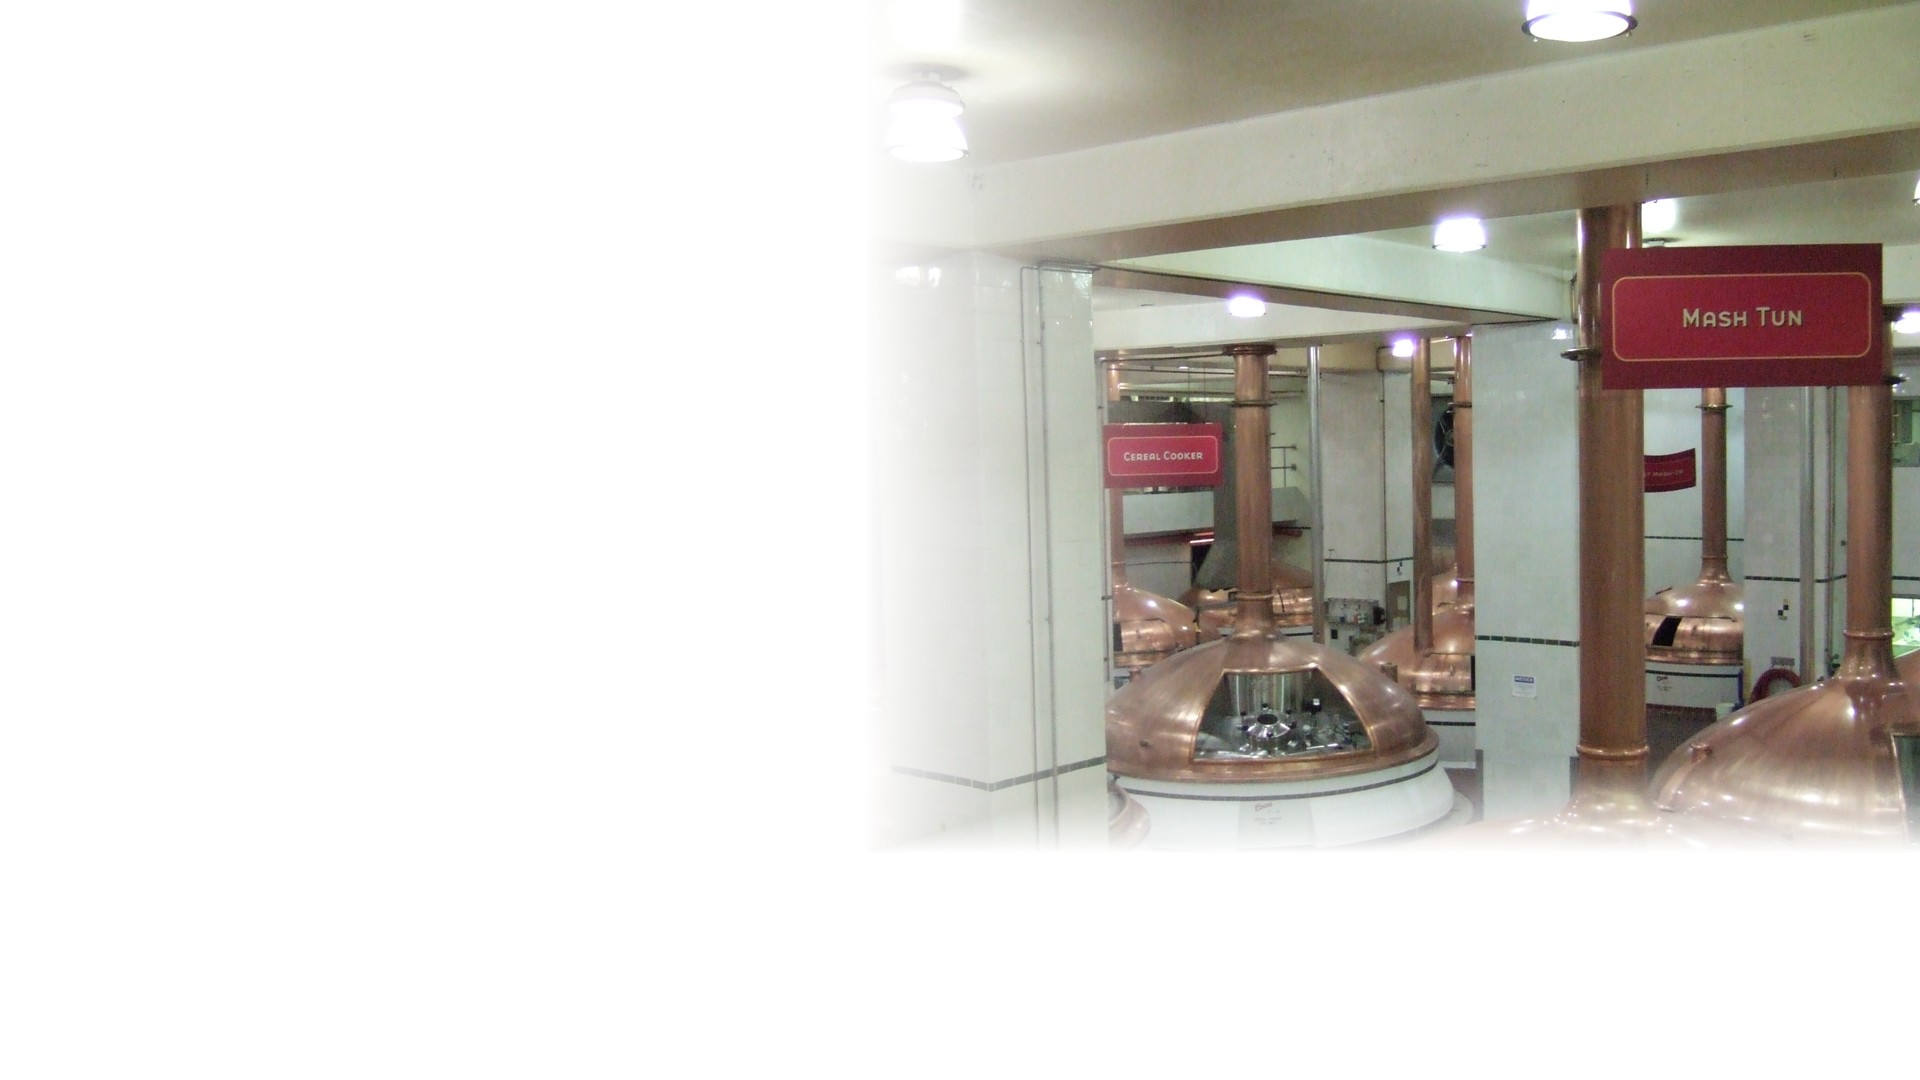
\includegraphics[width=\paperwidth,height=\paperheight]{imgs/verificadas/bg-pitch-brassagem.jpg}%
}
\begin{frame}[t]{Pitch}
  \vspace{0.1cm}
  \parbox{0.45\textwidth}{%
    {\Large\bfseries Vídeo do pitch}\\[0.15cm]
    {\small Duração: 1 min 48 s}\\[0.25cm]
    \qrcode[height=2.0cm]{https://youtu.be/4jTvFUkc8AM}\\[0.1cm]
    {\scriptsize\texttt{youtu.be/4jTvFUkc8AM}\footnotemark[1]}}

  \vfill

  \legenda{2}{sala de brassagem com tinas de mosturação.\footnotemark[2]}
  \footnotetext[1]{EQUIPE MASH. Projeto Integrador: Pitch. YouTube (não listado), 03/11/2026. Acesso em: 11 nov. 2026.}
  \footnotetext[2]{SDGJAKE. Coors Mash Tun. Wikimedia Commons, 2006. CC BY-SA 3.0. Recortada e com degradê branco.}
\end{frame}
}

% ============================================================
% 04 - PROBLEMATIZAÇÃO
% ============================================================
\section{Problematização}
\begin{frame}[t]{Problematização}
  \begin{columns}[T]
    \begin{column}{0.55\textwidth}
      \begin{itemize}
        \item O teste do iodo é \textbf{qualitativo}: indica amido que ainda reage com o iodo. Não mede açúcares.
        \item A leitura é a olho: tons intermediários, luz e reflexos mudam a cor vista.
        \item Temperatura e tempo mostram a rampa cumprida, não a conversão do amido\footnotemark[1].
        \item Sem data, hora e temperatura junto da leitura, comparar lotes fica difícil.
      \end{itemize}
    \end{column}
    \begin{column}{0.41\textwidth}
      \centering
      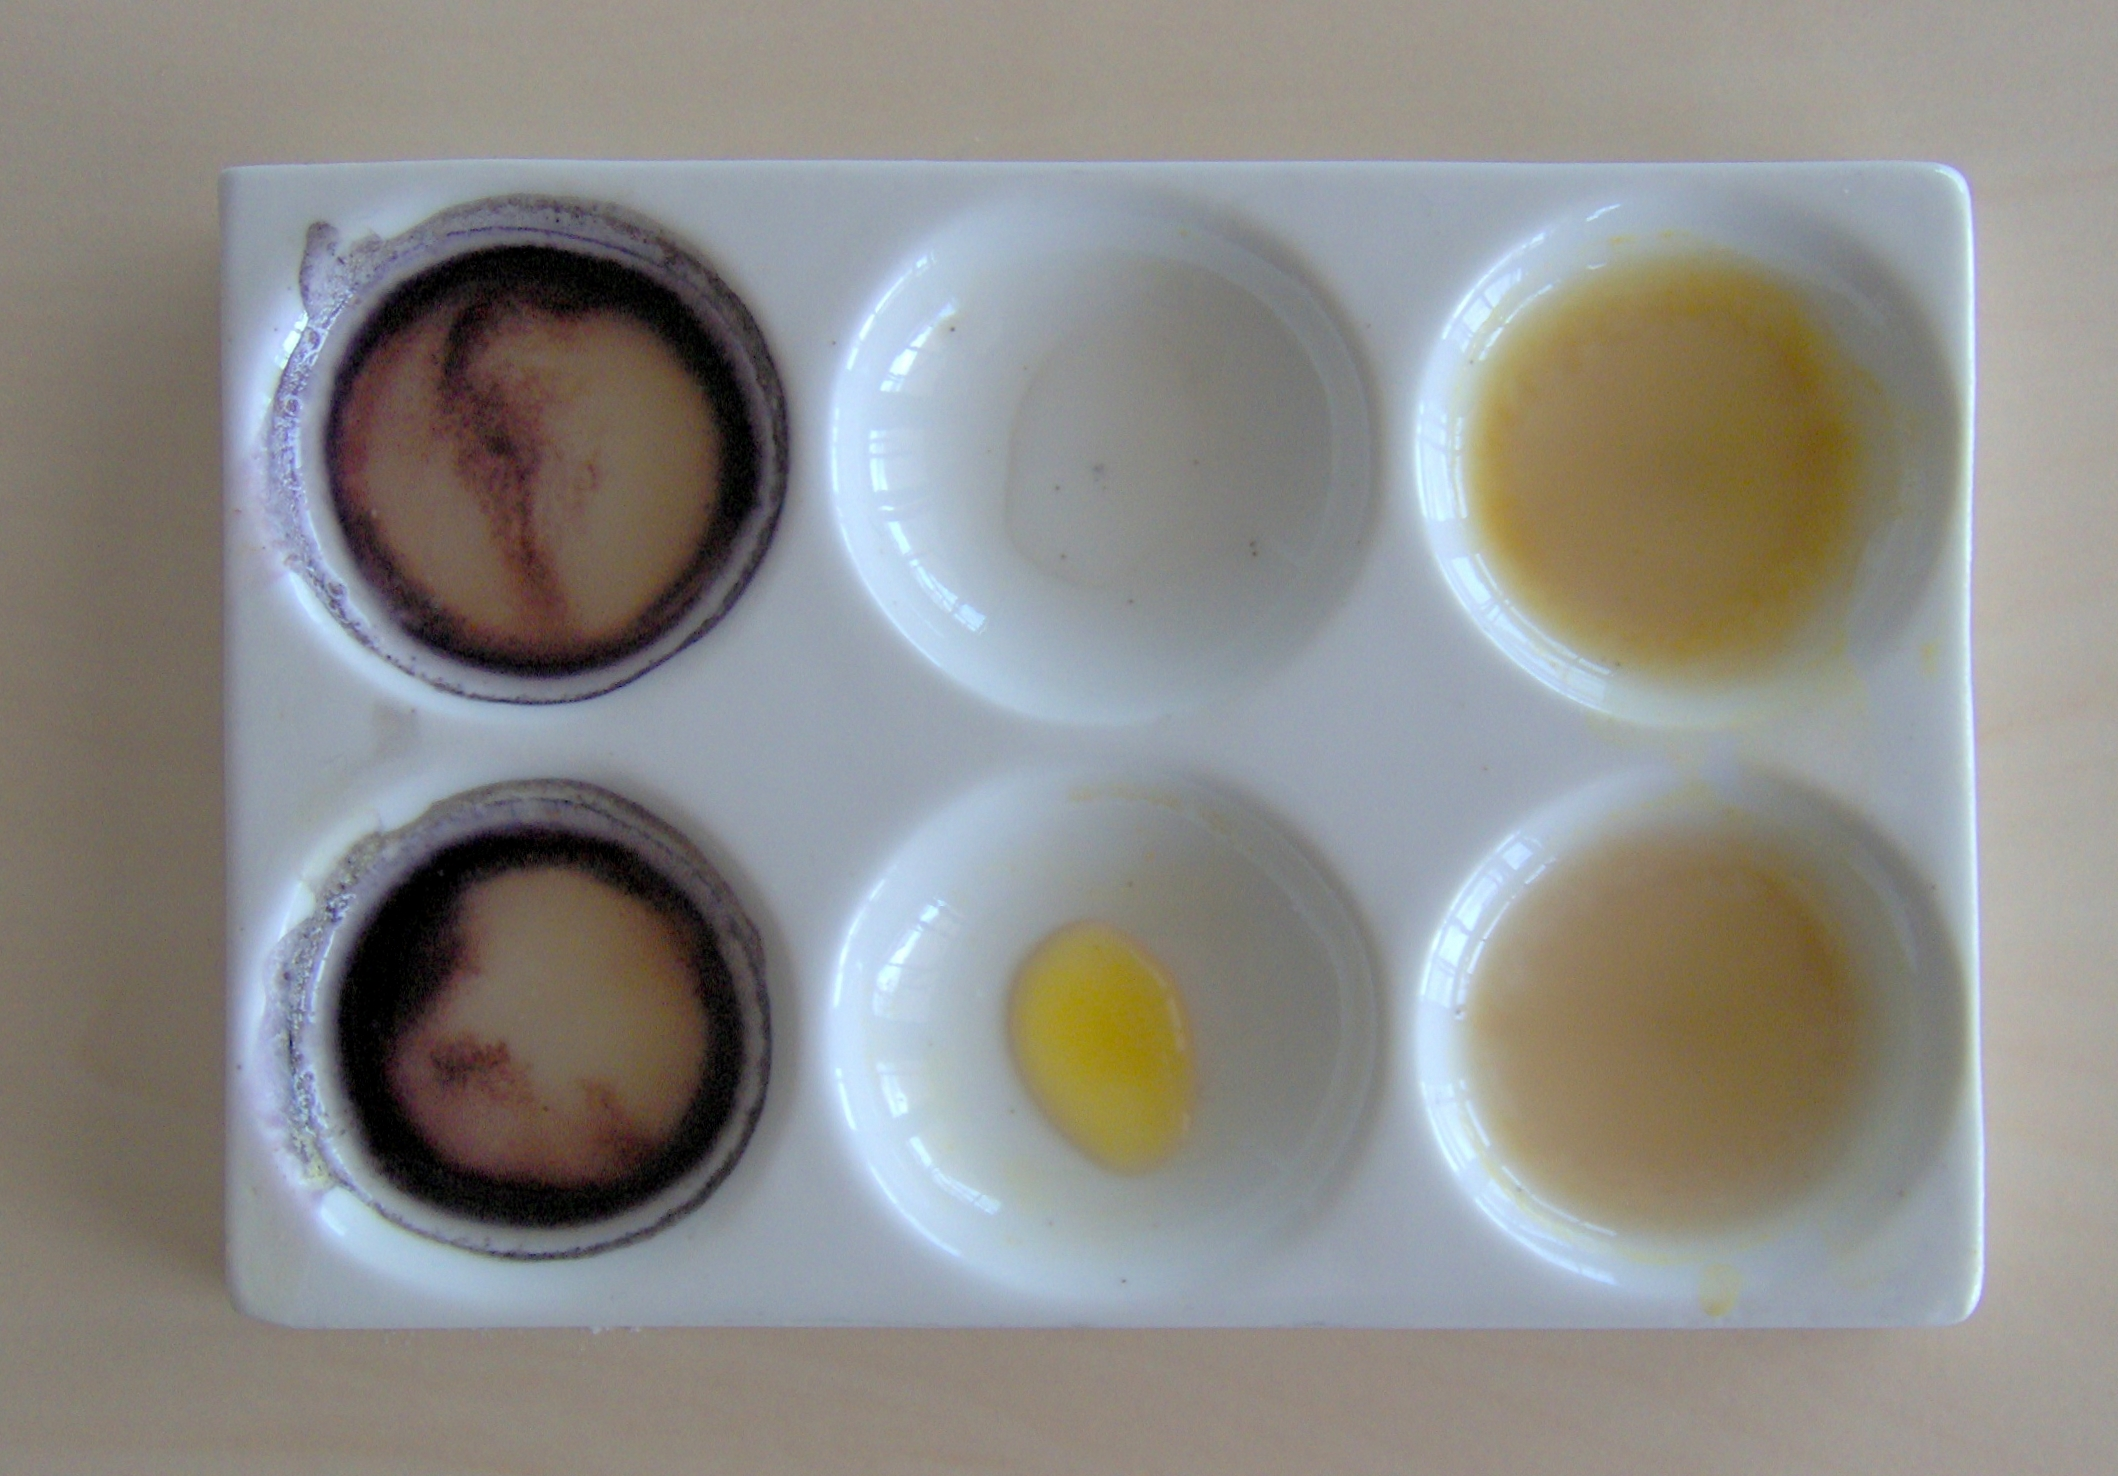
\includegraphics[width=0.82\linewidth]{imgs/verificadas/fig1-jodprobe.jpg}\par
      \vspace{0.1cm}
      \raggedright
      \legenda{3}{teste do iodo em mostura: amido presente (esquerda) e convertido (direita), segundo o autor.\footnotemark[2]}
    \end{column}
  \end{columns}
  \footnotetext[1]{HORNINK, G. G. \emph{Princípios da Produção Cervejeira e as Enzimas na Mosturação}. 2. ed. Alfenas-MG, 2024.}
  \footnotetext[2]{FLO SORG. Jodprobe.jpg. Wikimedia Commons, 2006. Domínio público. \url{https://commons.wikimedia.org/wiki/File:Jodprobe.jpg}.}
\end{frame}

% ============================================================
% 05 - ESTADO DA ARTE
% ============================================================
\section{Estado da Arte}
\begin{frame}[t]{Estado da Arte}
  \begin{center}
    \footnotesize
    \renewcommand{\arraystretch}{1.0}
    \begin{tabular}{|>{\raggedright\arraybackslash}p{2.4cm}|>{\raggedright\arraybackslash}p{3.6cm}|>{\raggedright\arraybackslash}p{3.0cm}|>{\raggedright\arraybackslash}p{2.9cm}|}
      \hline
      \textbf{Trabalho} & \textbf{Contribuição} & \textbf{Limitação} & \textbf{Lacuna para o Mash} \\
      \hline
      Parizotto\footnotemark[1] & Controle PI de rampas; sobressinal 1,7\% e 2,54\% & Sem monitoramento bioquímico do amido & Controle térmico sem leitura do iodo \\
      \hline
      Almeida e Ribeiro\footnotemark[2] & Teste do iodo no início e no fim da mosturação & Leitura visual, sem registro digital & Falta leitura padronizada \\
      \hline
      Nyarko et al.\footnotemark[3] & Estabilidade da espuma por segmentação HSV & Reflexos e autofoco em RGB & Não trata o teste do iodo \\
      \hline
      Li et al.\footnotemark[4] & Amido em tabaco pela cor RGB, com \textbf{antrona} & Erro médio de 3,83\% entre iluminações & Não é iodo nem mosto \\
      \hline
    \end{tabular}
  \end{center}
  {\small\textbf{Lacuna:} nenhum dos trabalhos analisados une leitura padronizada do iodo e registro do processo.}
  \footnotetext[1]{PARIZOTTO, G. Automação de equipamento para fabricação de cerveja artesanal. TCC (Engenharia Elétrica), UTFPR, 2017.}
  \footnotetext[2]{ALMEIDA, L. V.; RIBEIRO, J. S. \emph{Revista Ifes Ciência}, v. 10, n. 2, p. 1--11, 2024.}
  \footnotetext[3]{NYARKO, E. K. et al. \emph{Fermentation}, v. 7, n. 2, p. 46, 2021.}
  \footnotetext[4]{LI, W. et al. \emph{Scientific Reports}, v. 15, p. 6689, 2025.}
\end{frame}

% ============================================================
% 06 - OBJETIVO
% ============================================================
\section{Objetivo}
{
\usebackgroundtemplate{%
  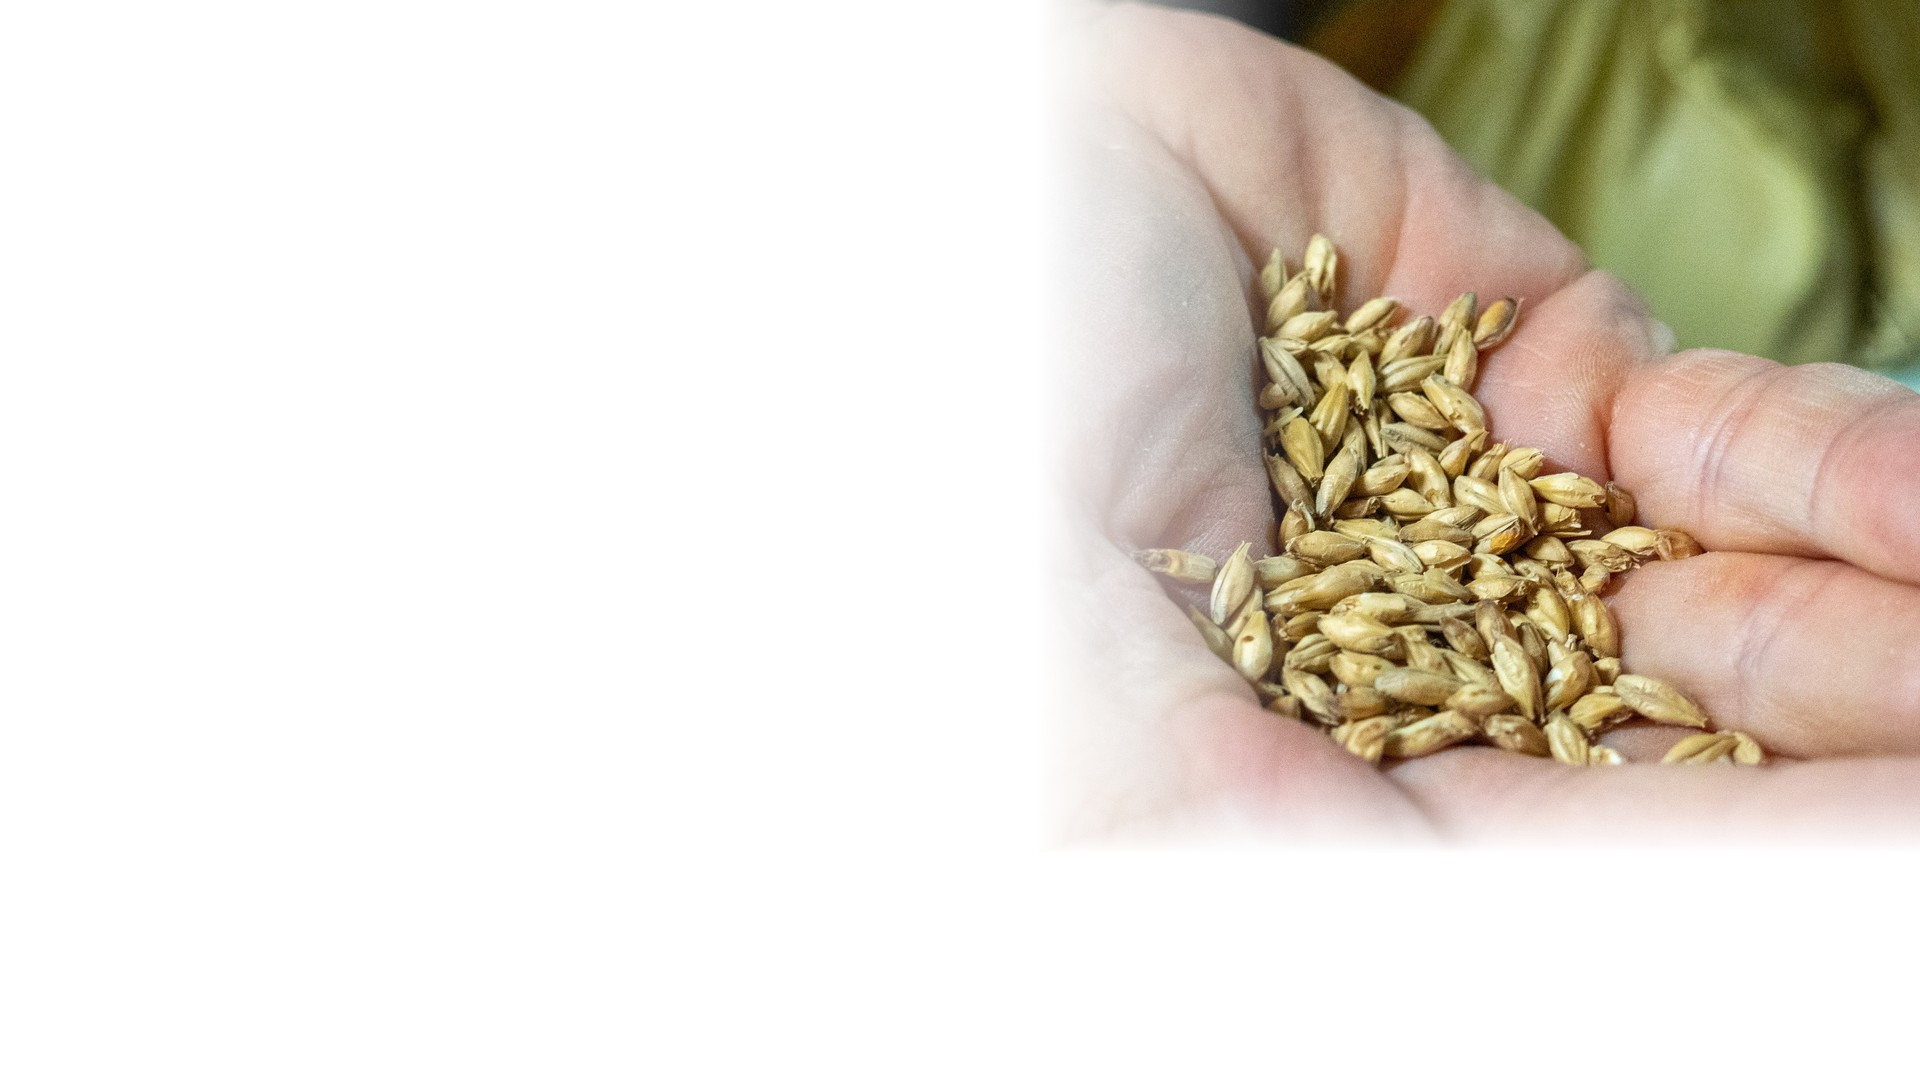
\includegraphics[width=\paperwidth,height=\paperheight]{imgs/verificadas/bg-objetivo-malte.jpg}%
}
\begin{frame}[t]{Objetivo}
  \begin{itemize}
    \item \parbox[t]{0.54\textwidth}{\raggedright \textbf{Geral}: plataforma que acompanhe a mosturação e automatize a leitura do teste do iodo\footnotemark[1]}
    \item \parbox[t]{0.50\textwidth}{\raggedright \textbf{Específicos}:}
    \begin{itemize}
      \item \parbox[t]{0.52\textwidth}{\raggedright Receitas, rampas e lotes \implementado}
      \item \parbox[t]{0.52\textwidth}{\raggedright Fluxo do teste do iodo na interface \demonstrador}
      \item \parbox[t]{0.52\textwidth}{\raggedright Captura padronizada e classificação em três classes \planejado}
      \item \parbox[t]{0.52\textwidth}{\raggedright Resultado ligado ao lote e método avaliado \planejado}
    \end{itemize}
  \end{itemize}

  \vfill

  \legenda{4}{malte, a fonte do amido convertido na mosturação.\footnotemark[2]}
  \footnotetext[1]{Artigo do projeto Mash (2026), seção 2.}
  \footnotetext[2]{NORALAMBERT. Carapils Malt for Brewing. Wikimedia Commons, 2021. CC BY-SA 4.0. Recortada e com degradê branco.}
\end{frame}
}

% ============================================================
% 07 - METODOLOGIA
% ============================================================
\section{Metodologia}
\begin{frame}[t]{Metodologia}
  \begin{columns}[T]
    \begin{column}{0.62\textwidth}
      \small
      Quatro módulos: aquisição, processamento de imagem, registro da mosturação e interface.
      \begin{enumerate}
        \item Literatura e requisitos \concluido
        \item Receitas, rampas e lotes \implementado
        \item Captura padronizada e controles \planejado
        \item Análise de cores em HSV e CIELAB \planejado
        \item Três classes; imagem ruim: inconclusiva \planejado
      \end{enumerate}
    \end{column}
    \begin{column}{0.34\textwidth}
      \centering
      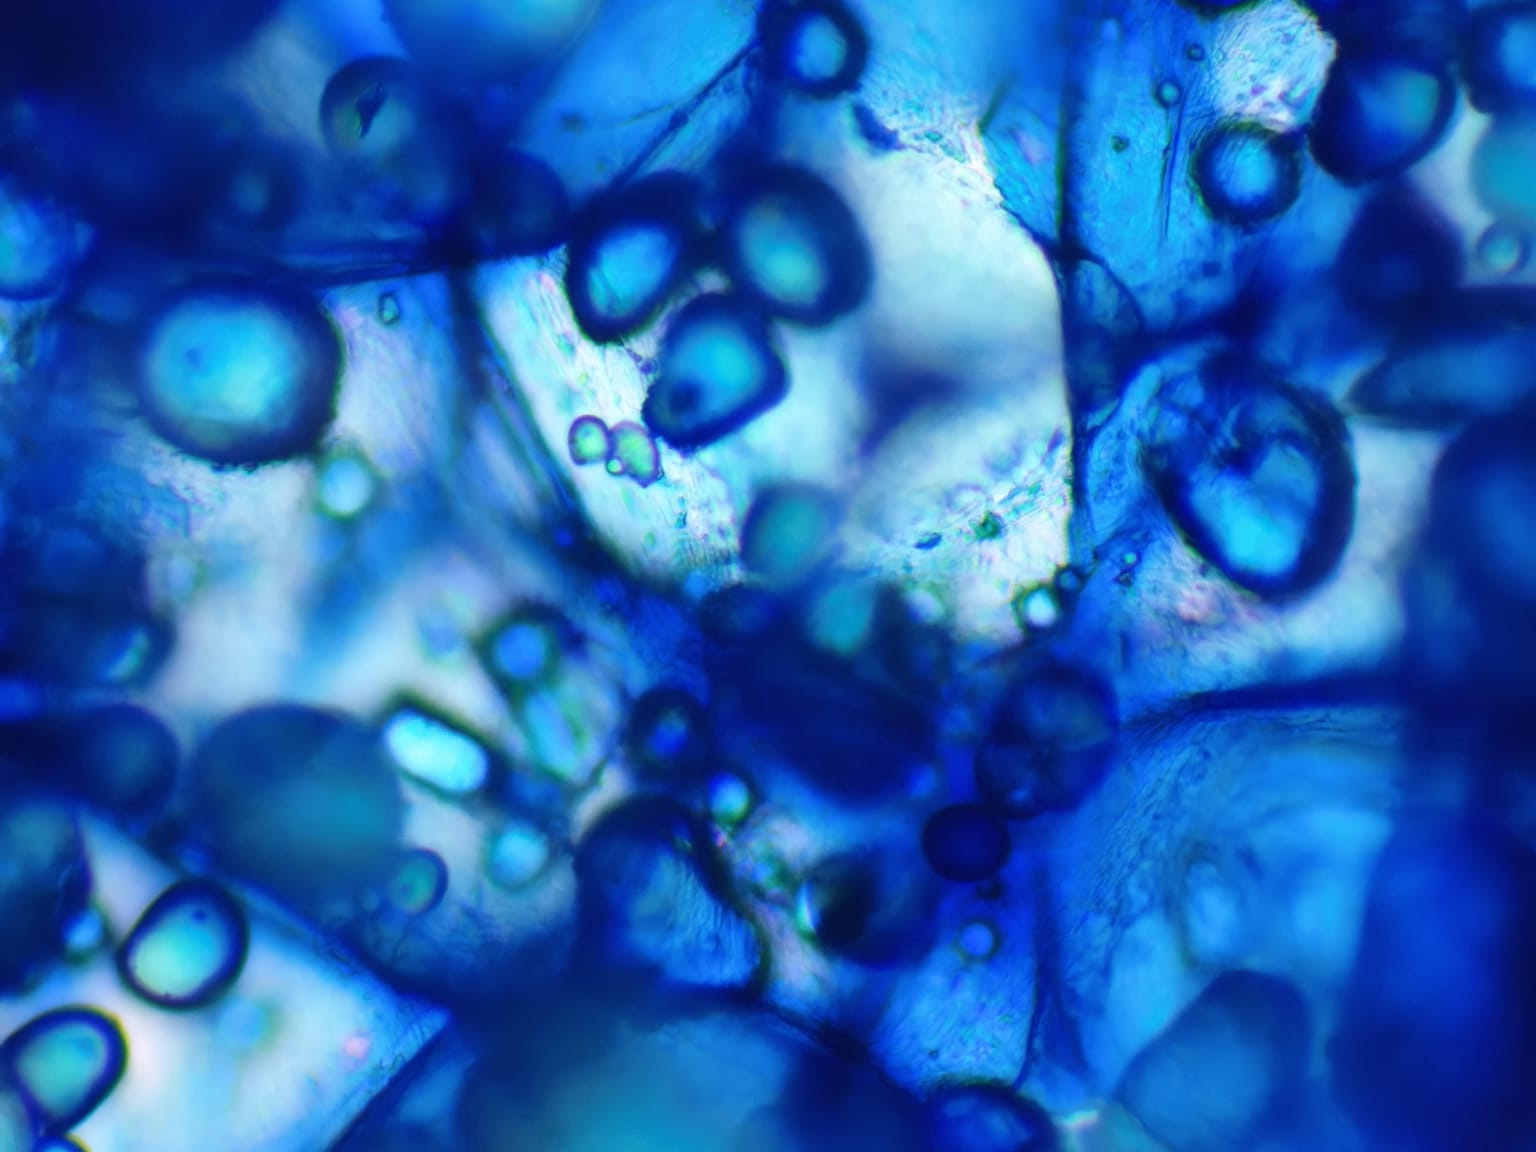
\includegraphics[width=0.80\linewidth]{imgs/verificadas/fig2-lugol-recorte-4x3.jpg}\par
      \vspace{0.1cm}
      \raggedright
      \legenda{5}{amido corado com iodo (Lugol), 400×.\footnotemark[1]}
    \end{column}
  \end{columns}
  \footnotetext[1]{ALEROMJAR1403. Potato amyloplasts stained with Lugol's solution. Wikimedia Commons, 2025. CC0. Recorte 4:3.}
\end{frame}

\begin{frame}[t]{Metodologia: tecnologias e validação}
  \begin{columns}[T]
    \begin{column}{0.48\textwidth}
      \textbf{Tecnologias}
      \begin{itemize}
        \item Plataforma: Node.js/Express, Sequelize/MySQL e React/Next.js \implementado
        \item OpenCV.js no navegador, separado do sistema \provaconceito
        \item Análise real: Python e OpenCV\footnotemark[1] \planejado
      \end{itemize}
      {\small Também: Tailwind CSS e acesso com Argon2id e JWT \implementado}
    \end{column}
    \begin{column}{0.48\textwidth}
      \textbf{Plano de validação} \planejado
      \begin{itemize}
        \item Comparar com controles e dois avaliadores
        \item Medir acertos e erros: matriz de confusão e acurácia\footnotemark[2]
        \item Registrar inconclusivos e repetibilidade
        \item Validar em bancada antes do ambiente real
      \end{itemize}
    \end{column}
  \end{columns}
  \footnotetext[1]{BRADSKI, G. The OpenCV Library. \emph{Dr. Dobb's Journal of Software Tools}, v. 25, n. 11, p. 120--125, 2000.}
  \footnotetext[2]{Acurácia calculada só entre classificações conclusivas; inconclusivos reportados à parte. Artigo do projeto Mash (2026), seções 2 e 4.6; critérios a reavaliar após o estudo piloto.}
\end{frame}

% ============================================================
% 08 - APRESENTAÇÃO PRÁTICA (demonstração ao vivo, 4 min 15 s)
% ============================================================
\section{Apresentação prática}
{
\usebackgroundtemplate{%
  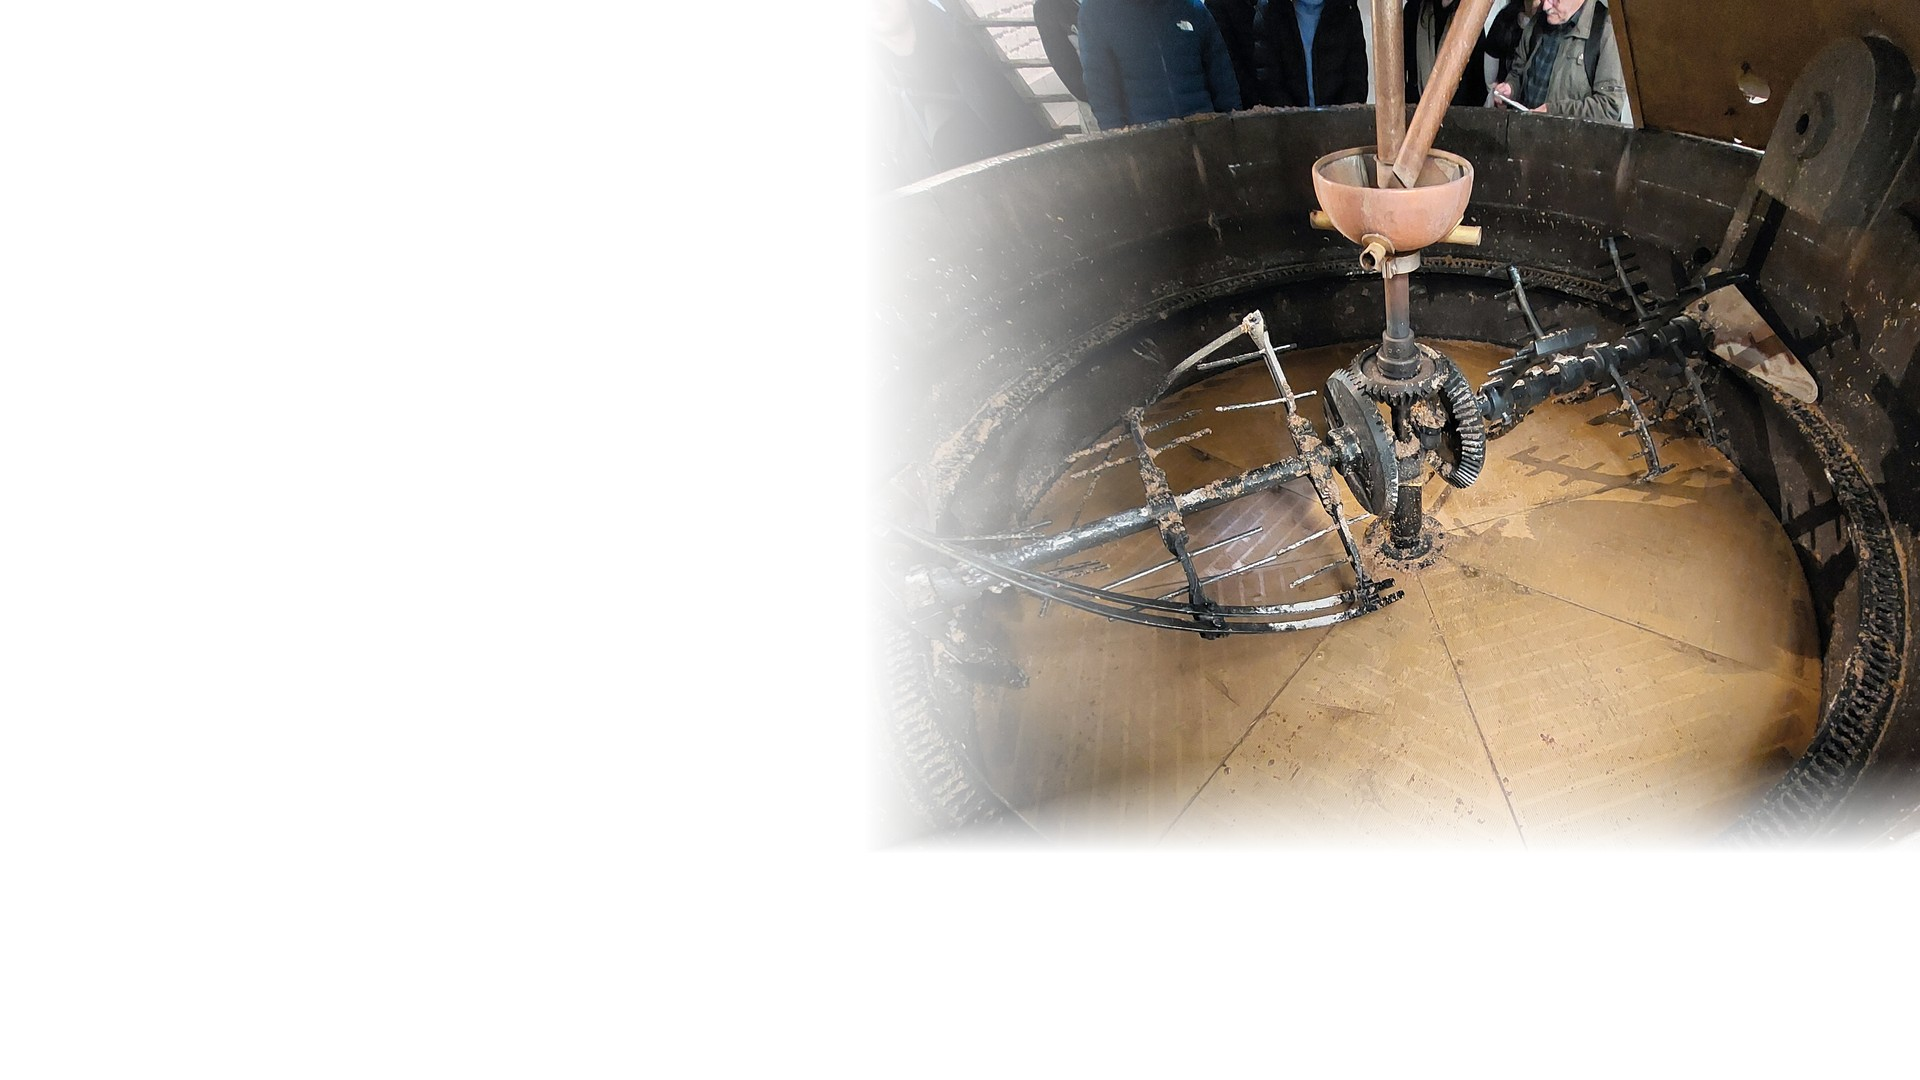
\includegraphics[width=\paperwidth,height=\paperheight]{imgs/verificadas/bg-pratica-tina.jpg}%
}
\begin{frame}[t]{Apresentação prática}
  \vspace{0.1cm}
  {\Large\bfseries Demonstração ao vivo}\par\vspace{0.1cm}
  {\small 4 min 15 s, no sistema em funcionamento}

  \vspace{0.15cm}
  \begin{enumerate}
    \item \parbox[t]{0.42\textwidth}{\raggedright Login e receita com rampas de temperatura}
    \item \parbox[t]{0.42\textwidth}{\raggedright Lote vinculado à receita}
    \item \parbox[t]{0.42\textwidth}{\raggedright Fluxo do teste do iodo \demonstrador}
  \end{enumerate}

  \vspace{0.1cm}
  \parbox{0.44\textwidth}{\raggedright\scriptsize No teste do iodo, as leituras são simuladas: a tela não classifica fotos reais.}

  \vfill

  \legenda{6}{tina de mosturação de uma cervejaria.\footnotemark[1]}
  \footnotetext[1]{CANLI, E. Brasserie Cantillon's mash tun 2024. Wikimedia Commons, 2024. CC BY-SA 4.0. Recortada e com degradê branco.}
\end{frame}
}

% Encerramento (dentro da seção Apresentação prática; manual, item 2.5)
\begin{frame}
  \vspace{0.3cm}
  \begin{center}
    
\includegraphics[height=1.9cm]{imgs/produto/logo-mash.png}\par
    {\tiny\textbf{Figura 1}: logomarca do Mash (repetida).}\par
    \vspace{0.4cm}
    {\Large\bfseries Obrigado!}\par
    \vspace{0.2cm}
    {\small Agradecemos à banca avaliadora e à plateia pela atenção.}\par
    {\small Estamos à disposição para perguntas.}
  \end{center}
\end{frame}

\end{document}
